\title{Representing High-Dimensional Decision Boundaries from Support Vector Machines and Neighborhood Graphs}
\author{Dan Maljovec}
\date{\today}

\documentclass[12pt]{article}
\usepackage{graphicx}
\usepackage{amsmath}
\DeclareMathOperator*{\argmin}{arg\,min}

\begin{document}
\maketitle

\begin{abstract}
This is a brief outline detailing work to be done for completion of my
dissertation.
%
For the final section of my dissertation, I have proposed to investigate methods
for extracting decision boundaries in various dimension spaces. 
%
Specifically, I aim at targeting spaces ranging from 2-10 dimensions.
%
The format of this document begins with an introduction of the problem posed by
my collaborators and I at Idaho National Laboratory.
%
Next, I will review the literature of techniques addressing this and similar
problems which include methods employing a support vector machine or a graph
either inherit or imposed on the data.
%
Following this discussion, I will discuss the advantages and drawbacks to each
of the proposed techniques and follow on with the novel contributions which I
believe will provide better explicit representations of the boundary surface
existing between two classes of data.
%
I conclude this article with a proposed set of experiments that will exercise
the various baseline and novel methods on their ability to extract low error,
well-spaced, and complete decision boundaries in various dimensions.
\end{abstract}

\section{Introduction}

Idaho National Laboratory has made a concerted effort toward developing what
they call the Risk-Informed Safety Margins Characterization (RISMC)
pathway~\cite{YoungbloodMousseauKelly2010}.
%
An integral part of this pathway is characterizing a simulation space into areas
of system failure and system success.
%
Consider analysis of a nuclear power plant simulation under duress such as in
the station blackout scenario~\cite{MaljovecLiuWang2015}.
%
Under this pathway, scientists want to understand the threshold, or what is
often called the limit surface or decision boundary, existing in the simulation
input space that differentiates between system recovery and system failure.
%
With such information at hand, they can begin to design safety systems that push
orthogonally against this decision boundary in such a way that maximizes the
safety tolerance while limiting the cost of the system.

Standard classification techniques implicitly encode a decision boundary, also
known as a decision boundary, by allowing users to query unrealized locations in
the domain space for a label.
%
Such methods are, in a sense, black boxes with great predictive power, but a
user cannot directly understand the shape of the decision boundary or extract
it from the model.
%
A common goal in reliability engineering is to understand when and how a system
fails and being able to avoid such circumstances.
%
Furthermore, when constructing surrogate models for high-dimensional and
computationally expensive models it is often beneficial to perform sampling in
an adaptive fashion.
%
The decision boundary from the current surrogate represents the area of least
predictive confidence of the model and so refining near this area is oftentimes
beneficial.
%
For this reason, a better understanding of the global/local shape and gradient
along the decision boundary can inform practitioners of the stability of the
system under study.
%
Therefore, being able to explicitly represent the decision boundary occurring
between system failure and normal operation provides scientists with information
crucial to subsequent analysis of such systems.

\section{Related work}

\subsection{Decision Boundary Estimation and Extraction}

\begin{itemize}
	\item \cite{DiamantiniPotena2007} - Overview of various methods for
	estimating decision boundaries (Good pointer to other relevant works)
	\item  \cite{Fukunaga1990,ParkParkPardalos2004} - Linear Discriminant
	Analysis (Canonical Analysis)
	\begin{itemize}
		\item Finds a projection that best ``splits'' the two classes
		\item (Fails if data is not separable in the low-dimensional setting)
		\item ``minimizes within class scatter and maximizes between class
		scatter.''
	\end{itemize}
	\item \cite{LeeLandgrebe1993} - Decision boundary and normal vectors are
	estimated numerically from non-parametric classifiers
	\begin{itemize}
		\item  (e.g., Parzen density estimator (used in the paper), kNN, neural
		networks)
		\item Uses nearest (euclidean distance) neighbor edge to associate a
		decision boundary sample for each point.
	\end{itemize}
	\item \cite{LeeLandgrebe1997} - Artifical neural networks (ANNs)
	(Multi-layer perceptron (MLP)) to do the same type of extraction
	as~\cite{LeeLandgrebe1993}
	\item \cite{GoLee2003} improves~\cite{LeeLandgrebe1997} by computing normal
	analytically
	\item \cite{ZhangLiu2005} - [IMPORTANT] - SVM for optimal decision boundary
	\begin{itemize}
		\item (Quadratic optimization cost limits the amount of data)
		\item Limitation of DBA -- cannot accurately estimate the boundary in
		high-dimensions
		\item Goal is to overcome small sample size situations
		\item Support vectors are used to analytically find points on the
		decision boundary by looking at their nearest neigbhors on the other
		side (solve for $\alpha$: $h(s) = h(\alpha z_1 + (1 - \alpha) z_2)$)
	\end{itemize}
	\item \cite{DiamantiniPotena2006} - [IMPORTANT] - Labeled Vector Quantizier
	(LVQ) for optimal decision boundary 
	\begin{itemize}
		\item (As good or better results than SVM for cheaper) 
	\end{itemize}
	\item \cite{WooLee2017} -Something more contemporary?
	\begin{itemize}
		\item
	\end{itemize}
\end{itemize}

\subsection{Papers on neighborhood graphs}

\begin{itemize}
	\item $\theta$-graphs, Yao Graphs, and $\gamma$-graphs
	\item \cite{CardinalColletteLangerman2009} - Properties and proofs of empty region
	graphs in the plane (2D)
	\begin{itemize}
		\item Introduces the ``pacman'' generalization of the $\beta$-skeleton
		that can represent both the lune and circle-based RNG.
		\item Also looks at infinite slabs which resemble the $\beta_p$-skeleton
		where either $\beta=\infty$ or the limit as $\beta$ and $p$ approach
		$0$.
	\end{itemize}
	\item \cite{JaromczykToussaint1992} - Survey of neighborhood graphs
	\item \cite{JaromczykKowaluk1987} - Discusses computation of RNG using
	$L_p$-metrics for arbitrary dimension.
	\item \cite{KowalukMajewska2014} - Investigating $\beta$-skeletons in $L_p$ spaces
	where $1 < p < \infty$
	\item \cite{CorreaLindstrom2011} - Demonstrates effectiveness of Beta
	skeleton and diamond graph
	\item Is there anywhere that points out diamond graph is $L_1$-norm?
	\item \cite{MaljovecSahaLindstrom2013} - Another study similar to the one
	above
	\item \cite{AggarwalHinneburgKeim2001} - Demonstrates why $L_p$-norms where
	$p<2$ are useful for nearest neighbor queries
	\item \cite{ZhangKing2002b} - Here the $\beta$-skeleton is used to compute
	the support vectors of a support vector machine, however it reduces the
	accuracy of the SVM.
	\begin{itemize}
		\item We differ here because we want to extract the decision boundary
		from the identified SVM not use it to restrict our SVM search.
		\item \cite{ZhangKing2002a} describes how the algorithm works
	\end{itemize}
	\item \cite{GotoIshidaUchida2015} - [IMPORTANT] Similar to above only the RNG is used to
	compute the support vectors.
	\begin{itemize}
		\item Uses memoization to speed up RNG computation.
		\item Calls boundary point on RNG ``bridge'' vectors.
	\end{itemize}
	\item \cite{BennettBredensteiner2000} draws connection between convex hulls and svms
	\item \cite{ZengXuXie2008} - selecting convex hull samples in the feature space for SVM training (SebSVM - smallest enclosing ball)
	\item \cite{BhattacharyaPoulsenToussaint1981} - first paper to use graph editing, only for nearest neighbor classification not SVM.
\end{itemize}

% \subsection{Papers on visualizing SVMs}

% \begin{itemize}
% 	\item Most worked in 4D or lower.
% \end{itemize}

\section{Support Vector Machines}

Support Vector Machines (SVMs) were first introduced as a means of binary
classification via a linear separator~\cite{VapnikLerner1963}.
%
In the classical case, a hyperplane is used to divide two classes of points
where a subset of the original data is used to determine this hyperplane.
%
The specific subset of data used are known as the \emph{support vectors} and can
intuitively be thought of as the points closest to the boundary separating the
two classes.
%
Using the support vectors, we can construct the equation of the separating
hyperplane, $S_0: 0 = \mathbf{w} \cdot \mathbf{x} - b$ by constructing an
optimality criteria that the hyperplane has a maximal distance to the support
vectors and the fewest number of misclassified points (in the case where the
data is not linearly separable).
%
Figure~\ref{fig:svmExample} shows an annotated example of the support vector
machine applied to a dataset that is linearly separable.

\begin{figure}[!ht]
  \centering
  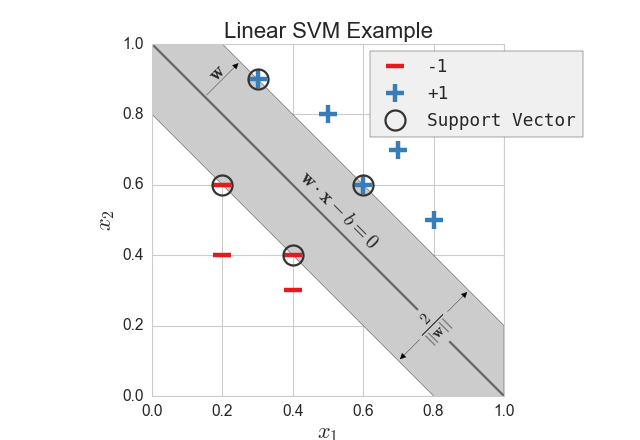
\includegraphics[width=0.85\textwidth]{figs/chap3/svmExample}
  \caption[Linear Support Vector Machine Example]{A two-dimensional example
  dataset showing the linear separator, margin, and support vectors of a trivial
  classification problem.}
  \label{fig:svmExample}
\end{figure}

We can see from Figure~\ref{fig:svmExample} that the support vectors of each
class define hyperplanes that are parallel to $S_0$, namely $S_{-}$ and $S_{+}$
which are set to be defined by the equations $-1 = \mathbf{w} \cdot \mathbf{x} -
b$ and $1 = \mathbf{w} \cdot \mathbf{x} - b$, respectively.
%
The shaded region bounded by the separating hyperplanes, $S_{-}$ and $S_{+}$,
is known as the \emph{margin} and represents the area we seek to maximize.
%
The width of the margin is inversely proportional to the norm of the separating
hyperplane coefficients, $\mathbf{w}$.
%
Therefore, by minimizing $||\mathbf{w}||$ according to the constraint that our
data lies on the correct side of the margin, we obtain the optimal separating
hyperplane.

If we define our class labels to be $y_i: y_i \in \{-1,1\}$, then we can rewrite
the constraints in a single equation: $y_i(\mathbf{w} \cdot \mathbf{x_i} - b )
\geq 1$ for $i=1,...,n$ where $n$ is the number of support vectors.
%
In the case where the data is not linearly separable in the original space, we
can either relax our constraint to include a soft margin that allows points to
be misclassified~\cite{CortesVapnik1995} and/or the data can be transformed into
a feature space where it is linearly separable~\cite{BoserGuyonVapnik1992}.

\subsubsection{Soft Margin SVM}

To instantiate a soft margin, we replace the constraint function with a loss
function so that our optimization problem penalizes equations that misclassify
points.
%
The \emph{hinge loss} function is often used for such purposes, and it is
defined in Equation~\ref{eq:hingeLoss}.
%
\begin{equation}
l(\mathbf{x_i},y_i) = \max(0,1-y_i(\mathbf{w} \cdot \mathbf{x_i} - b))
\label{eq:hingeLoss}
\end{equation}
%
Note that for correctly classified data, the hinge loss function will return
zero and the value increases the farther a misclassified point is from $S_-$
(for $y_i=-1$) or $S_+$ (for $y_i=1$).
%
We then combine this hinge loss over all of the support vectors with the
original minimization criteria on $||\mathbf{w}||$ to give the minimization
problem in Equation~\ref{eq:svmSoftMargin}.
\begin{equation}
\argmin_{\mathbf{w},b}\frac{1}{n}\sum_{i=1}^n \left(l(\mathbf{x_i},y_i)\right) +
\lambda ||\mathbf{w}||^2
\label{eq:svmSoftMargin}
\end{equation}

The $\lambda$ in the above optimization represents a postive real number and
allows a user to appropriately weight how important the size of the margin
should be in comparison to the correctness of classification.
%
As $\lambda$ decreases in magnitude, the behavior of the SVM will tend toward
the hard-margin case described above.

\subsubsection{Kernel SVM}

Consider the example shown in Figure~\ref{fig:kernelSvmExample}.
%
The image on the left represents the data in the original data space, and it is
clear that there does not exist a line that can separate the two classes.
%
However, we can note that by applying a transformation operator, $K$ on the
original data, we can transform it into a space where the data is linearly
separable as shown in the right image.
%
In this case, we have kept the dimensionality the same ($d=2$), but we have
transformed our cartesian coordinates ($x_1$ and $x_2$) into polar coordinates
($r$ and $theta$).
%
This is the main concept behind kernel-based SVMs where often the data is
projected into a higher dimensional feature space.

\begin{figure}[!ht]
  \centering
  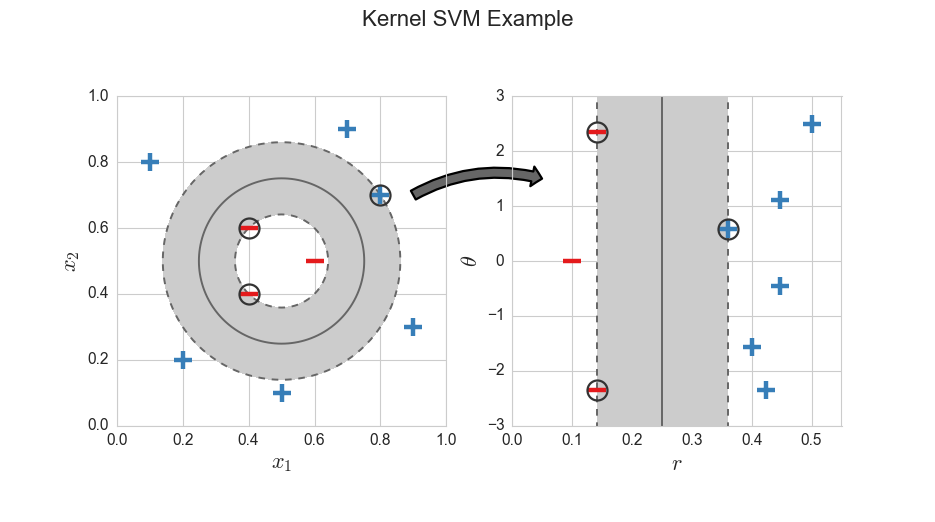
\includegraphics[width=0.85\textwidth]{figs/chap3/kernelSvmExample}
  \caption[Kernel Support Vector Machine Example]{A two-dimensional example
  dataset is transformed into a different space where it can be linearly
  separated and the support vector algorithm acts on the transformed space.}
  \label{fig:kernelSvmExample}
\end{figure}

When applying a kernel on the data, the same optimization process can be applied
in the higher dimensional feature space in order to determine the maximum-margin
linear separator in the feature space~\cite{BoserGuyonVapnik1992}.
%
Common kernels include polynomial, radial basis, sigmoid, and hyperbolic tangent
functions.
%
It should be noted that as opposed to transforming the data into a fixed
dimension space these methods instead transform the data into a feature space
whose dimensionality is dependent on the number of training samples.

The resulting optimization of all of the described SVM methods is $O(n^2)$ with
respect to the training size and the computation time is not affected by the
dimensionality of the original space.
%
However, it is worth noting that as dimensionality increases, the out-of-sample
error can become a problem which requires more training data to counterbalance.

\section{Labeled Vector Quantizers}

I need to read more about these, but my suspicion is that these are similar to
SVMs instead using ``coding'' vectors rather than support vectors.

\section{Empty Region Graphs}

The previous methods described by Diamantini and
Potena~\cite{DiamantiniPotena2007}, use only a nearest neighbor edge to
determine the decision boundary leaving much to be desired in being able to
extract the topology of the decision boundary.
%
In order to understand the decision boundary more completely, it is beneficial
to us to use a denser graph.
%
Correa and Lindstrom~\cite{CorreaLindstrom2011} demonstrated the effectiveness
of a class of graphs known as \emph{empty region graphs}...

In this work, the diamond graph performed as well or better than all of the
other graphs in many instances.
%
Note, that the canonical diamond graph ($\theta=\frac{\pi}{4}$) is actually a
special case of the Gabriel graph where the $L_1$-norm unit ball is used around
the edge as opposed to the $L_2$-norm used by the Gabriel graph.
%
Furthermore, Aggarwal et al.~\cite{AggarwalHinneburgKeim2001} prove the relative
contrast of the $L_2$-norm is sub-optimal in higher dimensional spaces.
%
For this reason I would like to investigate the use of other norms in
constructing the decision boundary.

\begin{figure}[!ht]
  \centering
  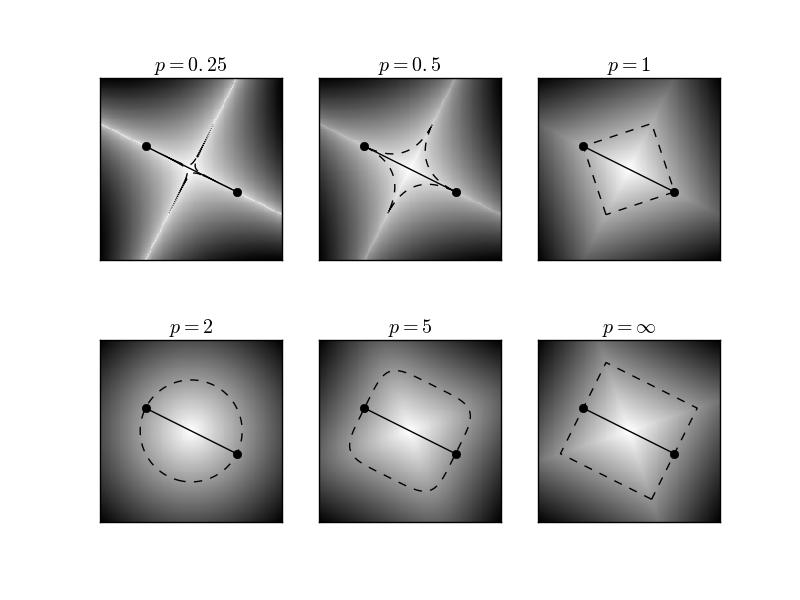
\includegraphics[width=0.9\textwidth]{figs/chap6/emptyRegions}
  \caption[Gabriel graph empty regions using various $L_p$-norms]{A
  two-dimensional edge and the shape of its empty region for the Gabriel graph
  case ($\beta=1$) given various values of $p$.}
  \label{fig:ergs}
\end{figure}

I believe these can be computed relatively cheaply in arbitrary dimension using
the correct parameterization. See Figure~\ref{fig:ergParameterization}.

\begin{figure}[!ht]
  \centering
  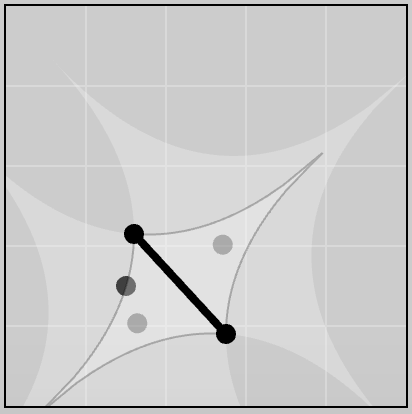
\includegraphics[width=0.4\textwidth]{figs/chap6/bskeleton}
  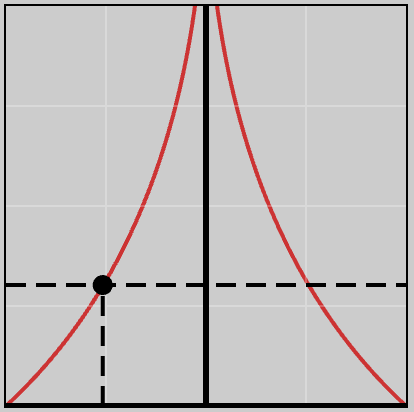
\includegraphics[width=0.4\textwidth]{figs/chap6/bskeletonParameter}
  \caption[Example edge test where $\beta=.4$ and $p=0.5$. The space can be
  parameterized by the edge.]{TODO}
  \label{fig:ergParameterization}
\end{figure}

\section{Proposed Extraction Methodology}

In the various works on decision boundary feature extraction laid out by
Diamantini and Potena~\cite{DiamantiniPotena2007}, each method relies on a
nearest neighbor search in order to interpolate points that lie on the limit
surface.

We can see even in the simple Figure~\ref{fig:kernelSvmExample}, that this would
not yield an accurate representation of the decision boundary.
%
Therefore, I propose to use empty region graphs defined over the entire training
dataset in order to extract the decision boundary.
%
Furthermore, I propose the $\beta_p$-skeleton which allows for more flexibility
in defining the empty region around each edge.

[INSERT PICTURES OF WHAT THESE LOOK LIKE HERE]

\section{Proposed Experimentation}

Three metrics:
\begin{enumerate}
	\item \textbf{Error} - How close are the identified points to the true
	decision boundary? 
	\begin{itemize}
		\item Given we have an analytic function to evaluate.
		\item Residual: $|f(x)-t|$, where $f$ is the analytic function, $x$ is
		the identified point, and $t$ is the specified isovalue.
		\item Length of path to decision boundary using gradient descent?
	\end{itemize}
	\item \textbf{Coverage} - Do we capture the whole domain?
	\begin{itemize}
		\item Given known bounds on each dimension can we verfiy that the span
		of the decision boundary is reached in each example?
	\end{itemize}
	\item \textbf{Efficieny} - How many points were extracted and at what
	fidelity?
	\begin{itemize}
		\item Points should be well-spaced, but may be more concentrated in
		areas of high curvature.
		\item Blue noise like property on manifold?
		\item Evaluate dispersion of data.
		\item A denser graph will give more points, but they may exhibit clustering around specific areas. Do these clusterings make sense (i.e., areas of high curvature)?
	\end{itemize}
\end{enumerate}

In order to test each of these properties, we will need functions that scale in dimensionality and exercise each of these properties.

\begin{itemize}
	\item \textbf{Zero curvature} - hyperplane 
	\item \textbf{Constant curvature} - Circular/ellipsoidal
	\item \textbf{Variable curvature} - Sine-like
	\item \textbf{Discontinuous curvature} - Sharp corner or box
\end{itemize}

\begin{itemize}
	\item \textbf{Dimension spanning} - hyperplane
	\item \textbf{Non-dimension spanning} - circular and sharp corner/box
	\item \textbf{Anisotropic} - ellipsoidal
	\item \textbf{Multiple connected components} - circular/ellipsoidal
	\item \textbf{Void/Hole} - annulus/salomon
\end{itemize}

\bibliographystyle{abbrv}
\bibliography{thesis}

\end{document}
